\begin{problem}{\#1 (21 points)}
    Let \(\Sigma = \{a,b\}\)
    \begin{enumerate}[label=\textbf{\alph*)}]
        \item Build an FA that accepts only those words that do not end in \(ab\).
        \item Build an FA that accepts only the language of all words with \(b\) as the second letter.
        Find the regular expression for the language.
        \item Build an FA that accepts only those words that have more than four letters.
        \item Build an FA that accepts only those words that have fewer than four letters.
        \item Build an FA that accepts only those words with exactly four letters.
        \item Build an FA that accepts only those words that begin or end with a double letter.
    \end{enumerate}
\end{problem}
\vspace{2em}
\begin{solution}
    \begin{enumerate}[label=\textbf{\alph*)}]
        \item 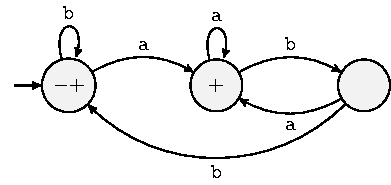
\includegraphics[]{figures/answer/Answer1-A.pdf}
        \\
        \item 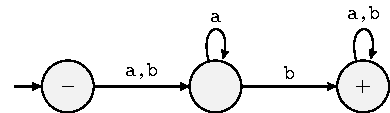
\includegraphics[]{figures/answer/Answer1-B.pdf}
        \newpage
        \item 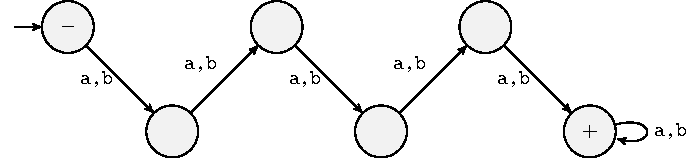
\includegraphics[]{figures/answer/Answer1-C.pdf}
        \\
        \item 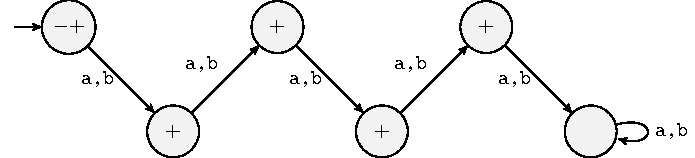
\includegraphics[]{figures/answer/Answer1-D.pdf}
        \\
        \item 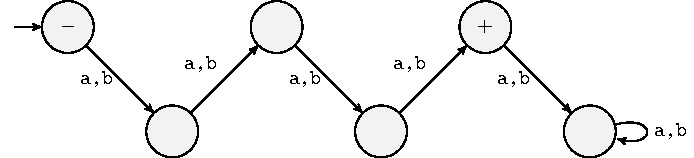
\includegraphics[]{figures/answer/Answer1-E.pdf}
        \\
        \item 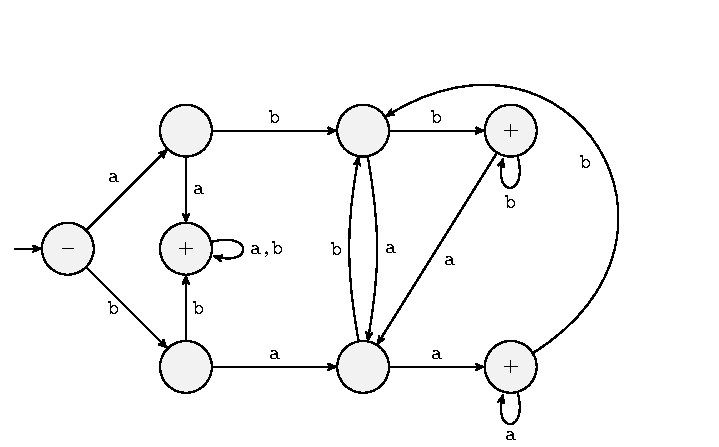
\includegraphics[]{figures/answer/Answer1-F.pdf}
    \end{enumerate}
\end{solution}

\begin{problem}{\#2 (15 points)}
    Describe in English words the definition of the language and give a regular expression for the language accepted by each of the following FAs and TGs.
    \begin{enumerate}[label=\textbf{\alph*)}]
        \item 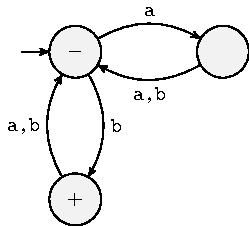
\includegraphics[width=15em]{figures/question/Question2-A.pdf}
        \item 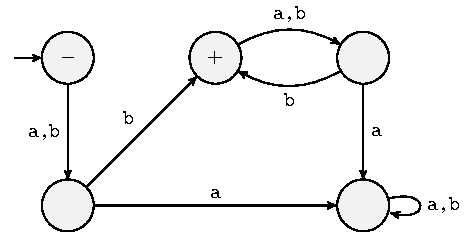
\includegraphics[width=25em]{figures/question/Question2-B.pdf}
        \item 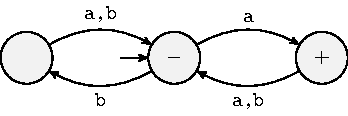
\includegraphics[width=20em]{figures/question/Question2-C.pdf}
        \item 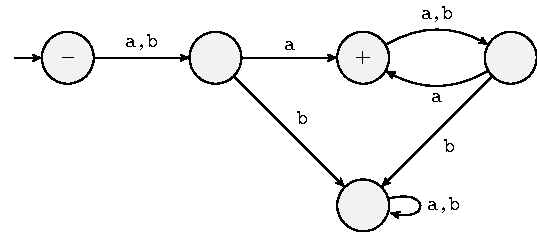
\includegraphics[width=30em]{figures/question/Question2-D.pdf}
        \item 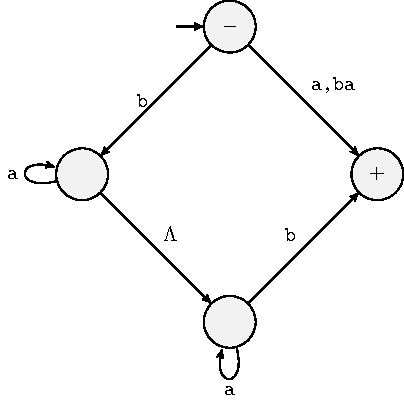
\includegraphics[width=25em]{figures/question/Question2-E.pdf}
    \end{enumerate}
\end{problem}
\vspace{2em}
\begin{solution}
    \begin{enumerate}[label=\textbf{\alph*)}]
        \item This FA accepts all odd length words that end with a \(b\).
        The regular expression of this FA is: \(((a+b)(a+b))^*b\)
        \item This FA accepts all words that do not have the sequence \(aa\) or \(ba\) and ends with \(b\).
        The regular expression of this FA is: \((a+b)b((a+b)b)^*\)
        \item This FA accepts all words of odd length that end with an \(a\).
        The regular expression of this FA is: \(a+((a+b)(a+b)a)^*\).
        \item This FA accepts all words of even length that end with \(a\) and do not have the sequence \(bb\).
        The regular expression of this FA is: \((a+b)a((a+b)a)^*\)
        \item This TG accepts the words \(a,ba\) and \(ba \ldots\ ab\) with any number of \(a\)'s between.
    \end{enumerate}
\end{solution}

\begin{problem}{\#3 (15 points)}
    For each of the FAs and TGs in Problem 2, build a transition graph that accepts the same language but has fewer states.
\end{problem}
\vspace{2em}
\begin{solution}
    \begin{enumerate}[label=\textbf{\alph*)}]
        \item 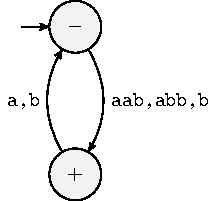
\includegraphics[width=12em]{figures/answer/Answer3-A.pdf}
        \item 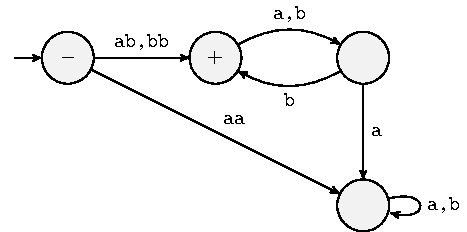
\includegraphics[width=25em]{figures/answer/Answer3-B.pdf}
        \item 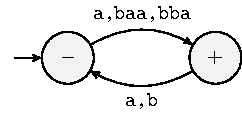
\includegraphics[width=12em]{figures/answer/Answer3-C.pdf}
        \item 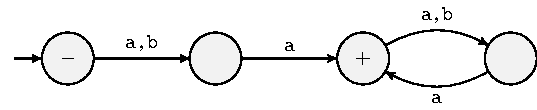
\includegraphics[width=25em]{figures/answer/Answer3-D.pdf}
        \item 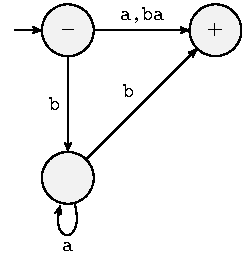
\includegraphics[width=15em]{figures/answer/Answer3-E.pdf}
    \end{enumerate}
\end{solution}